\documentclass[tikz,border=10pt]{standalone} % https://tikz.jp/doraemon/

\begin{document}

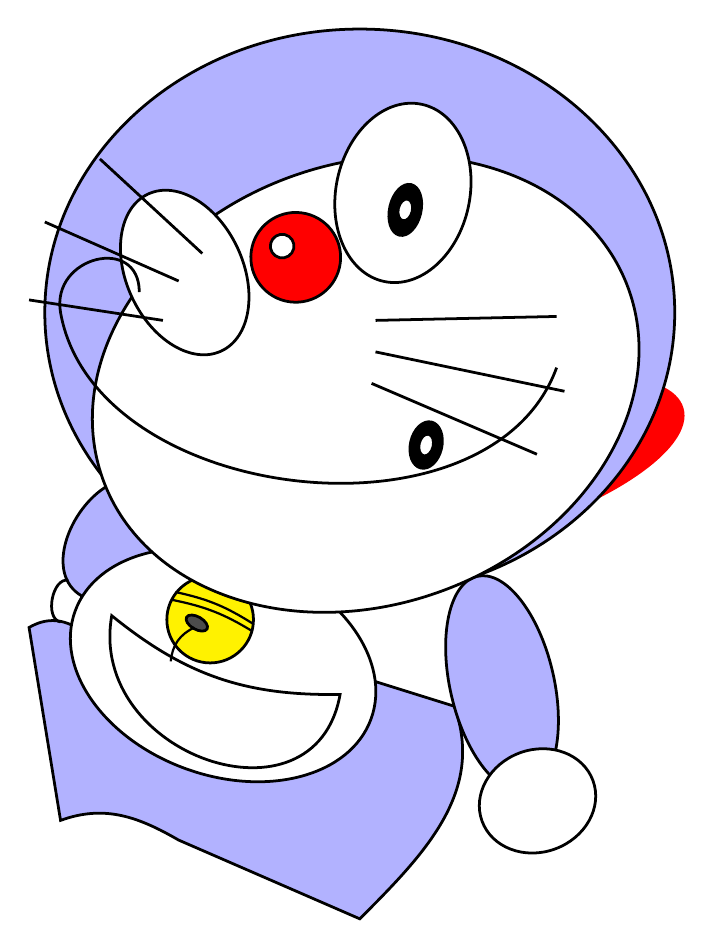
\begin{tikzpicture}[draw, line width=1pt, even odd rule]

% Corps
\filldraw[fill=blue!30] (1.2,-5) to[out=290, in=45] (0,-7.7)
  -- (-2.3,-6.7) to[out=150, in=20] (-3.8,-6.45)
  -- (-4.2,-4) to[out=30, in=150] (-3.6,-4)
  -- (-3.53,-3.6) to[out=150, in=210] (-3.2,-2.2) -- (-2,-4) --cycle;

% Poche
\filldraw[fill=white, rotate=-20] (-0.1,-4.8) ellipse (2 and 1.4);
\draw (-0.25,-4.85) to[out=260, in=260, looseness=1.5]
  (-3.15,-3.85) to[bend right=20] cycle;

% Ombre sous la poche
\filldraw[fill=blue!30, rotate=13] (0.7,-5) ellipse (0.66 and 1.4);
\filldraw[fill=white, rotate=20] (0,-6.6) ellipse (0.75 and 0.65);

% Détail de la poche
\draw (-3.7,-3.4) to [bend right=90] (-3.8,-3.93);

% Col rouge
\filldraw[rotate=16, red] (1.0,-2.3) ellipse (2.6 and 0.9);

% Clochette jaune
\filldraw[fill=yellow] (-1.9,-3.9) circle (0.55);

% Ombre sur la clochette
\filldraw[fill=black!70, rotate=-30] (0.18,-4.45) ellipse (0.15 and 0.08);

% Détails sur la clochette
\draw[thick] (-1.36,-4.05) to[bend right=10] (-2.38,-3.65);
\draw[thick] (-1.36,-3.95) to[bend right=10] (-2.34,-3.55);
\draw[thick] (-2.1,-4) to[bend right=30] (-2.4,-4.43);

% Tête
\filldraw[fill=blue!30] ellipse (4 and 3.6);

% Visage blanc
\filldraw[rotate=20,fill=white] (-0.24,-0.88) ellipse (3.55 and 2.8);

% Yeux
\draw[rotate=25, fill=white] (-1.8,1.4) ellipse (0.74 and 1.1);
\draw[rotate=-12, fill=white] (0.22,1.6) ellipse (0.85 and 1.15);

% Pupilles
\filldraw[rotate=-13]
  (1.2,-1.45) ellipse (0.2 and 0.3) ellipse (0.09 and 0.14)
  (0.27,1.4) ellipse (0.2 and 0.33) ellipse (0.09 and 0.14);

% Nez rouge
\filldraw[rotate=-13, fill=red] (-0.95,0.5) circle (0.57)
  ++(-0.2,0.1) circle (0.15);

% Moustaches
\draw (-2.8,0.26) to [out=90, in=100, looseness=1.8] (-3.8,0)
  to[out=280, in=250] (2.5,-0.7);
\draw (0.2,-0.1) --++ (2.3,0.05);
\draw (0.2,-0.5) --++ (2.4,-0.5);
\draw (0.15,-0.9) --++ (2.1,-0.9);
\draw (-2,0.75) --++ (-1.3,1.2);
\draw (-2.3,0.4) --++ (-1.7,0.75);
\draw (-2.5,-0.1) --++ (-1.7,0.26);

\end{tikzpicture}

\end{document}
